\documentclass[12pt]{article}


\usepackage{tikz}
\usetikzlibrary{calc}

\begin{document}
{
\def\vertexLabels{1}

            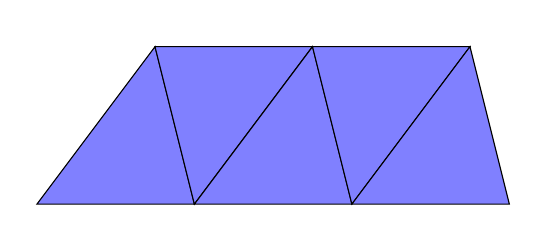
\begin{tikzpicture}
                \coordinate [label=below:\ifdefined \vertexLabels 1 \fi] (A) at (0,0);
                \coordinate [label=above:\ifdefined \vertexLabels 2 \fi] (B) at (1.5,2);
                \coordinate [label=below:\ifdefined \vertexLabels 3 \fi] (C) at (2,0);
                \coordinate [label=above:\ifdefined \vertexLabels 4 \fi] (D) at ($(B)+(C)$);
                \coordinate [label=below:\ifdefined \vertexLabels 5 \fi] (E) at ($2*(C)$);
                \coordinate [label=above:\ifdefined \vertexLabels 1 \fi] (F) at ($2*(C)+(B)$);
                \coordinate [label=below:\ifdefined \vertexLabels 2 \fi] (G) at ($3*(C)$);

                % Draw a face with vertices 1,2,3 and label 4 in the middle
                \def\drawFace#1#2#3#4{
                    \filldraw[fill=blue!50!white, draw=black] (#1) -- (#2) -- (#3) -- cycle;
                    \node at ($1/3*(#1)+1/3*(#2)+1/3*(#3)$) {#4};
                }
                
                \drawFace{A}{B}{C}{\ifdefined \vertexLabels I \fi}
                \drawFace{B}{C}{D}{\ifdefined \vertexLabels II \fi}
                \drawFace{C}{D}{E}{\ifdefined \vertexLabels III \fi}
                \drawFace{D}{E}{F}{\ifdefined \vertexLabels IV \fi}
                \drawFace{E}{F}{G}{\ifdefined \vertexLabels V \fi}
            \end{tikzpicture}
   }         
            
          \ifdefined \vertexLabels bla \fi
\end{document}